\documentclass[12pt]{article}
% Full article preamble (duplicated, no common file)
\usepackage{fontspec}
\usepackage[a4paper,margin=2.5cm,includefoot]{geometry}
\usepackage{polyglossia}
\usepackage{amsmath}
\usepackage{amssymb}
\usepackage{xcolor}
\usepackage{fancyhdr}
\usepackage{graphicx}
\usepackage{listings}
\usepackage[most]{tcolorbox}
\usepackage{pifont}
\usepackage{enumitem}
\usepackage{titlesec}
\usepackage[bottom]{footmisc}
\usepackage{titling}
\usepackage{minted}
\usepackage{etoolbox}
\usepackage{array}
\usepackage{extsizes}

\newfontfamily\emoji{Segoe UI Emoji}

\pagestyle{fancy}

\setmainlanguage[numerals=western]{arabic}
\setotherlanguage{english}
\newfontfamily\arabicfont[Script=Arabic]{Amiri}
\newfontfamily\arabicfonttt[Script=Arabic]{Courier New}

\lstset{
  language=[Sharp]C,
  numbers=left,
  stepnumber=1,
  numbersep=8pt,
  frame=single,
  basicstyle=\ttfamily\small,
  keywordstyle=\color{blue},
  stringstyle=\color{red},
  commentstyle=\color{green!50!black}
}

\newif\ifdetailed
\ifdefined\setdetailed
  \setdetailed
\fi

\newif\ifwithsols
\ifdefined\setwithsols
  \setwithsols
\fi

% unified tcolorboxes for articles
\tcbset{colback=white, colframe=black, fonttitle=\bfseries, boxrule=0.8pt}
\newtcolorbox{boxDef}[1][]{colback=blue!5!white,colframe=blue!75!black,
  title={{\emoji📘} تعريف\ifx\\#1\\\else ~#1\fi :}}
\newtcolorbox{boxExercise}[1][]{colback=cyan!5!white,colframe=cyan!70!black,
  title={{\emoji🧩} تمرين\ifx\\#1\\\else ~#1\fi :}}
\newtcolorbox{boxExample}[1][]{colback=yellow!5!white,colframe=orange!90!black,
  title={{\emoji📝} مثال\ifx\\#1\\\else ~#1\fi :}}
\newtcolorbox{boxNote}[1][]{colback=gray!10!white,colframe=black,
  title={{\emoji✨} ملاحظة\ifx\\#1\\\else ~#1\fi :}}
\newtcolorbox{boxAttention}[1][]{colback=magenta!10!white,colframe=magenta!80!black,
  title={{\emoji🔔} تنبيه\ifx\\#1\\\else ~#1\fi :}}
\newtcolorbox{boxWarning}[1][]{colback=red!5!white,colframe=red!75!black,
  title={{\emoji⚡} ملاحظة هامة\ifx\\#1\\\else ~#1\fi :}}
\newtcolorbox{boxSolution}[1][]{colback=green!5!white,colframe=green!60!black,
  title={{\emoji✅} حل\ifx\\#1\\\else ~#1\fi :}}
\newtcolorbox{boxSymbol}[1][]{colback=purple!5!white,colframe=purple!70!black,
  title={{\emoji🔣} رمز\ifx\\#1\\\else ~#1\fi :}}

\tcbset{simplecode/.style={ colback=gray!5, colframe=black!50, boxrule=0.4pt, arc=2pt, left=4pt,right=4pt,top=4pt,bottom=4pt}}
\newenvironment{boxCode}{\begin{tcolorbox}[simplecode]}{\end{tcolorbox}}

\newcolumntype{C}[1]{>{\centering\arraybackslash}p{#1}}

% redefine spaces after titles
\makeatletter
\renewcommand{\@maketitle}{%
  \begin{center}
    {\huge \bfseries \@title \par}%
    \vskip 0.2em % space between title and author
    {\large \@author \par}%
    % \vskip 0.2em % space between author and date
    % {\normalsize \@date \par}%
  \end{center}
}
\makeatother

\fancyhf{} % clear default
\fancypagestyle{plain}{
  \fancyhf{}
  \fancyhead[L]{مدرسة التسامح الشاملة}
  % \fancyhead[L]{
\includegraphics[height=1cm]{../../../images/logoTasamoh.png}}
  \fancyhead[R]{الأستاذ محمود اغبارية}
  \fancyfoot[C]{\thepage}
}

\fancyhead[L]{مدرسة التسامح الشاملة}
\fancyhead[R]{الأستاذ محمود اغبارية}
\fancyfoot[C]{\thepage}
% \date{\today}

\setcounter{tocdepth}{3} % only section subsection and subsubsection in TOC


% ----------------------


% \begin{document}

% \maketitle

% % \clearpage  % start TOC on a new page
% % \renewcommand{\contentsname}{جدول المحتويات}
% % \tableofcontents
% % \clearpage

% \part*{part 1} % the * prevents numbering
% \section*{مقدمة}
% \subsection*{مثال رياضي}
% \subsubsection*{مثال فرعي}
% \paragraph*{ paragraph 1}
% \subparagraph*{sub paragraph 1}

% \ifdetailed
% \begin{english}
% \begin{minted}{csharp}
% // C# Example
% \end{minted}
% \end{english}
% \fi

% OLD WAY
% \ifdetailed
% \begin{english}
% \begin{lstlisting}
% // C# Example
% \end{lstlisting}
% \end{english}
% \fi

% % 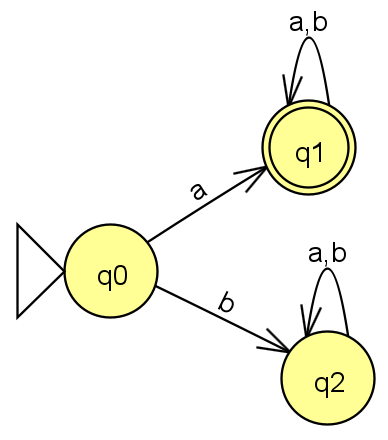
\includegraphics[width=0.2\textwidth]{../../../images/DFAs/ex1_q1.png}



% \vspace{3cm}
% \begin{flushleft}
% أرجو لكم وقتًا ممتعًا.

% الأستاذ محمود اغبارية.
% \end{flushleft}


% \end{document}


\title{وظيفة بيتية 4 للصف العاشر 10 - $\mathtt{if-statement}$}

\begin{document}

\maketitle
\thispagestyle{fancy}



\begin{enumerate}[itemsep=3em]

\item
موظف نشيط يستطيع ان يملأ نموذجا كل 10 دقائق، ويحصل على $7.2$ شيكل على كل نموذج. \\
أكتب مقطع برنامج يستقبل عدد النماذج التي يجب أن يملأها الموظف، على البرنامج أن يحسب ويطبع الوقت الذي يحتاجه الموظف لملء النماذج بالساعات والدقائق والأجر الذي سيحصل عليه بالنهاية.
\ifdetailed
\begin{boxExample}
\begin{english}
\begin{minted}{text}
Enter number of forms:
55
Time: 9 hours and 10 minutes
Wage: 396
\end{minted}
\end{english}
\end{boxExample}
\fi
\ifwithsols
\begin{boxSolution}
\begin{english}
\begin{minted}{csharp}
Console.Write("Enter number of forms: ");
int n = int.Parse(Console.ReadLine());
int totalMinutes = n * 10;
int hours = totalMinutes / 60;
int minutes = totalMinutes % 60;
double wage = n * 7.2;
Console.WriteLine($"Time: {hours} hours and {minutes} minutes");
Console.WriteLine($"Wage: {wage}");
\end{minted}
\end{english}
\end{boxSolution}
\clearpage
\fi

\item
اكتب مقطع برنامج يستقبل عددًا ثنائيّ المنزلة، ويطبع \textenglish{Yes} إذا كانت منزلتاه عددين متتاليين.
\ifdetailed
\begin{boxExample}[1]
\begin{english}
\begin{minted}{text}
Enter a two-digit number:
34
Yes
\end{minted}
\end{english}
\end{boxExample}
\begin{boxExample}[2]
\begin{english}
\begin{minted}{text}
Enter a two-digit number:
79
No
\end{minted}
\end{english}
\end{boxExample}
\ifwithsols
\begin{boxSolution}
\begin{english}
\begin{minted}{csharp}
Console.Write("Enter a two-digit number: ");
int n = int.Parse(Console.ReadLine());
int tens = n / 10;
int ones = n % 10;
if (Math.Abs(tens - ones) == 1)
{
    Console.WriteLine("Yes");
}
else
{
    Console.WriteLine("No");
}
\end{minted}
\end{english}
\end{boxSolution}
\fi
\clearpage
\fi

\item
اكتب مقطع برنامج يستقبل عددًا ثلاثي المنازل، ويطبع \textenglish{Palindrom} إذا كانت قراءته من اليمين إلى اليسار متطابقة مع قراءته من اليسار إلى اليمين.
\ifdetailed
\begin{boxExample}[1]
\begin{english}
\begin{minted}{text}
Enter a three-digit number:
121
Palindrom
\end{minted}
\end{english}
\end{boxExample}
\begin{boxExample}[2]
\begin{english}
\begin{minted}{text}
Enter a three-digit number:
123
\end{minted}
\end{english}
\end{boxExample}
\fi
\ifwithsols
\begin{boxSolution}
\begin{english}
\begin{minted}{csharp}
Console.Write("Enter a three-digit number: ");
int n = int.Parse(Console.ReadLine());
int hundreds = n / 100;
int ones = n % 10;
if (hundreds == ones)
{
    Console.WriteLine("Palindrom");
}
\end{minted}
\end{english}
\end{boxSolution}
\clearpage
\fi

\item
اكتب مقطع برنامج يستقبل ثلاثة أعداد، ويطبع العدد الأوسط بينها.
\ifdetailed
\begin{boxExample}
\begin{english}
\begin{minted}{text}
Enter three integers:
8
3
5
Middle = 5
\end{minted}
\end{english}
\end{boxExample}
\ifwithsols
\begin{boxSolution}
\begin{english}
\begin{minted}{csharp}
Console.WriteLine("Enter three integers:");
int a = int.Parse(Console.ReadLine());
int b = int.Parse(Console.ReadLine());
int c = int.Parse(Console.ReadLine());
int min = Math.Min(a, Math.Min(b, c));
int max = Math.Max(a, Math.Max(b, c));
int middle = a + b + c - min - max;
Console.WriteLine($"Middle = {middle}");
\end{minted}
\end{english}
\end{boxSolution}
\fi
\clearpage
\fi

\item
اكتب برنامجًا يستقبل 3 أعداد عشرية تمثل أطوال أضلاع مثلث. \\
على البرنامج أن يطبع نوع المثلث:
\begin{itemize}
    \item مثلث متساوي الأضلاع، إذا كانت كل أضلاعه متساوية
    \item مثلث متساوي الساقين إذا كان هناك ضلعان بالضبط متساويين.
    \item مثلث قائم الزاوية إذا كان المثلث يحقق قانون فيثاغورس: $a^2 + b^2 = c^2$ ($c$ هو الضلع الأطول بين الثلاثة.)
\end{itemize}
\ifdetailed
\begin{boxExample}[1]
\begin{english}
\begin{minted}{text}
Enter three sides:
3
3
3
Equilateral
\end{minted}
\end{english}
\end{boxExample}
\begin{boxExample}[2]
\begin{english}
\begin{minted}{text}
Enter three sides:
3
4
5
Right triangle
\end{minted}
\end{english}
\end{boxExample}
\fi
\ifwithsols
\begin{boxSolution}
\begin{english}
\begin{minted}{csharp}
Console.WriteLine("Enter three sides:");
double a = double.Parse(Console.ReadLine());
double b = double.Parse(Console.ReadLine());
double c = double.Parse(Console.ReadLine());
double x = a, y = b, z = c;
double[] arr = new double[] { x, y, z };
Array.Sort(arr);
x = arr[0]; y = arr[1]; z = arr[2];
if (x == y && y == z)
{
    Console.WriteLine("Equilateral");
}
else if (x == y || y == z || x == z)
{
    Console.WriteLine("Isosceles");
}
else if (Math.Abs(x * x + y * y - z * z) < 1e-9)
{
    Console.WriteLine("Right triangle");
}
else
{
    Console.WriteLine("Other");
}
\end{minted}
\end{english}
\end{boxSolution}
\fi

\clearpage
\item
اكتب مقطع برنامج يستقبل عددين عشريّين وعددًا صحيحًا،
ويقوم بعملية حسابية على النحو التالي:
\begin{itemize}
    \item إذا كان العدد الصحيح = 0، فإنه يطبع مجموع العددين العشريّين
    \item إذا كان العدد الصحيح = 1، فإنه يطبع الفرق بين العددين العشريّين (أي حاصل طرحهما بالقيمة المطلقة)
    \item إذا كان العدد الصحيح = 2، فإنه يطبع حاصل ضرب العددين العشريّين
    \item إذا كان العدد الصحيح = 3، فإنه يطبع حاصل قسمة العددين العشريّين (في هذه الحالة عليك التأكد أنّ العدد الثاني ليس 0، فإذا كان 0 عليك طباعة رسالة مناسبة.)
    \item في باقي الحالات يطبع العدد العشري الأول فقط.
\end{itemize}
\ifdetailed
\begin{boxExample}[1]
\begin{english}
\begin{minted}{text}
Enter two real numbers and a mode:
3.5
2.0
0
Result: 5.5
\end{minted}
\end{english}
\end{boxExample}
\begin{boxExample}[2]
\begin{english}
\begin{minted}{text}
Enter two real numbers and a mode:
3.5
2.0
1
Result: 1.5
\end{minted}
\end{english}
\end{boxExample}
\begin{boxExample}[2]
\begin{english}
\begin{minted}{text}
Enter two real numbers and a mode:
3.5
2.0
5
Result: 3.5
\end{minted}
\end{english}
\end{boxExample}
\fi

\ifwithsols
\begin{boxSolution}
\begin{english}
\begin{minted}{csharp}
Console.WriteLine("Enter two real numbers and a mode:");
double x = double.Parse(Console.ReadLine());
double y = double.Parse(Console.ReadLine());
int mode = int.Parse(Console.ReadLine());
if (mode == 0)
{
    Console.WriteLine($"Result: {x + y}");
}
else if (mode == 1)
{
    Console.WriteLine($"Result: {Math.Abs(x - y)}");
}
else if (mode == 2)
{
    Console.WriteLine($"Result: {x * y}");
}
else if (mode == 3)
{
    if (y == 0)
    {
        Console.WriteLine("ERROR: division by 0");
    }
    else
    {
        Console.WriteLine($"Result: {x / y}");
    }
}
else
{
    Console.WriteLine(x);
}
\end{minted}
\end{english}
\end{boxSolution}
\clearpage
\fi


\item
اكتب تعبيرًا منطقيا مناسبًا:
\begin{enumerate}
    \item العدد \textenglish{a} يقسم على العدد \textenglish{b} بدون باقٍ.
    \item \textbf{كل} الأعداد \textenglish{a, b, c} أكبر من 10.
    \item \textbf{على الأقل أحد} الأعداد \textenglish{a, b, c} أكبر من 10.
    \item \textbf{كل} الأعداد \textenglish{a, b, c} زوجية.
    \item من بين الأعداد \textenglish{a, b, c} هناك عددان أحدهما يقسم على الآخر بدون باقٍ. (افترض أنه لا يوجد عدد يساوي 0)
    \item العدد \textenglish{a} يقسم على 2 أو على 3 لكن ليس على كليهما.
\end{enumerate}
\ifwithsols
\begin{boxSolution}
\begin{english}
\begin{minted}{csharp}
(b % a == 0)


(a > 10) && (b > 10) && (c > 10)


(a > 10) || (b > 10) || (c > 10)


(a % 2 == 0) && (b % 2 == 0) && (c % 2 == 0)


(b % a == 0) || (c % a == 0) || (c % b == 0) ||
(a % b == 0) || (a % c == 0) || (b % c == 0)


((a % 2 != 0) && (a % 3 == 0)) || ((a % 2 == 0) && (a % 3 != 0))
\end{minted}
\end{english}
\end{boxSolution}
\clearpage
\fi

\item
معطى التعبير المنطقي التالي:
\begin{english}
\begin{minted}{csharp}
(x > 0) || (y%2==0) && (x+y > 10)
\end{minted}
\end{english}
لكل واحدة من قيم $x,y$ التالية،املأ الجدول بـ \textenglish{true} او \textenglish{false}:

\begin{center}
\begin{tabular}{|c|c|c|c|c|c|c|}
\hline
$x$ & $y$ & $x>0$ & $y \% 2 = 0$ & $x+y>10$ & النتيجة الكلية للتعبير \\
\hline
5  & 3  &  &  &  &  \\
\hline
$-2$ & 4  &  &  &  &  \\
\hline
$-2$ & 12 &  &  &  &  \\
\hline
$-5$ & 5  &  &  &  &  \\
\hline
3  & 20 &  &  &  &  \\
\hline
$-3$ & 15 &  &  &  &  \\
\hline
\end{tabular}
\end{center}
\textbf{انتبه لترتيب العمليات المنطقية.}
\ifwithsols
\begin{boxSolution}
\begin{center}
\begin{tabular}{|c|c|c|c|c|c|}
\hline
\large{$x$} & \large{$y$} & \large{$x>0$} & \large{$y \% 2 = 0$} & \large{$x+y>10$} & \large{\textenglish{result}} \\
\hline
5 & 3 & true & false & false & true \\
\hline
$-2$ & 4 & false & true & true & true \\
\hline
$-2$ & 12 & false & true & true & true \\
\hline
$-5$ & 5 & false & false & false & false \\
\hline
3 & 20 & true & false & true & true \\
\hline
$-3$ & 15 & false & false & true & false \\
\hline
\end{tabular}
\end{center}
\end{boxSolution}
\fi

\clearpage
\item
خرج الأستاذ خالد مع طلاب صفه إلى جولة قريبة من المدرسة. \\
طلب الأستاذ من الطلاب أن ينتظموا بشكل ثنائي، ولكن تبين أن أحد الطلاب بقي وحيداً. \\
فطلب الأستاذ من الطلاب أن ينتظموا بشكل ثلاثي، ولكن أيضا تبين أن أحد الطلاب بقي وحيداً. \\
فقرر الأستاذ أن ينتظم الطلاب بشكل رباعي، ولكن أيضا هذه المرة بقيت نفس المشكلة وبقي طالب وحيد. \\
اكتب مقطع برنامج يستقبل عددًا صحيحًا، ويطبع \textenglish{possible} إذا كان هذا العدد من الممكن أن يكون هو عدد طلاب صف الأستاذ خالد.
\ifdetailed
\begin{boxExample}
\begin{english}
\begin{minted}{text}
Enter class size:
25
possible
\end{minted}
\end{english}
\end{boxExample}
\fi
\ifwithsols
\begin{boxSolution}
\begin{english}
\begin{minted}{csharp}
Console.Write("Enter class size: ");
int n = int.Parse(Console.ReadLine());
if (n % 2 == 1 && n % 3 == 1 && n % 4 == 1)
{
    Console.WriteLine("possible");
}
\end{minted}
\end{english}
\end{boxSolution}
\fi

\end{enumerate}


\vspace{1cm}
\begin{flushleft}
أرجو لكم وقتًا ممتعًا.

الأستاذ محمود اغبارية.
\end{flushleft}


\end{document}